\chapter{本手法を用いた初段ミューオントリガーの性能評価}
実際にRun-3での性能について書く
位置依存性とか大量に

\section{機械学習を用いることによる CW 作成の効果}
\subsubsection{チェンバーごとのEfficiency}
\begin{figure}[tb]
  \centering
  \rule{8cm}{6cm}
  %\includegraphics[clip, width=14cm]{}
  \caption{チェンバーごとのEfficiency (1-48)}
  \label{fig:fit_def}
\end{figure}

\subsubsection{ミューオンの電荷に対する効果}

\begin{figure}[tb]
  \centering
  \rule{8cm}{6cm}
  %\includegraphics[clip, width=14cm]{}
  \caption{Rate}
  \label{fig:fit_def}
\end{figure}


\section{Run-3に向けた本手法のトリガー性能}
Date と MC でeffの比較
\begin{figure}[tb]
  \centering
  \rule{8cm}{6cm}
  \caption{Efficiency}
  \label{fig:fit_def}
\end{figure}

\subsection{トリガーレート}
Date と MC
\begin{figure}[tb]
  \centering
  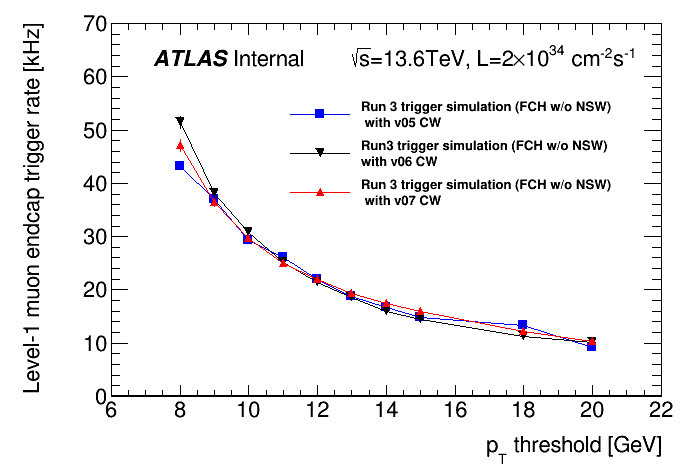
\includegraphics[clip, width=14cm]{fig/5/l1mue_rate_run3.png}
  \caption{Rate}
  \label{fig:fit_def}
\end{figure}

